\documentclass{article}
\usepackage{amsthm}
\usepackage{comment}
\usepackage{listings}
\usepackage{hyperref}
\newcommand\A{\mathbb{A}}
\newcommand\Epz{E\priveZE}
\newcommand\priveZE{∖\acco{0_E}}

\theoremstyle{remark}
\newtheorem*{note}{Note}
\excludecomment{note}

\begin{document}
ISEN Nantes CGSI2 \hfill à rendre pour le 10/11/2018
\title{Devoir libre n°4}
\maketitle

\section*{Simulation de variables aléatoires}

\paragraph{Principe}
Simuler une variable aléatoire, $X$, consiste à écrire un programme exécuter par la machine afin de réaliser virtuellement l'expérience
aléatoire aboutissant à une réalisation de la variable aléatoire, $X(\omega)$, où $\omega$ est une issue de l'expérience aléatoire. 
Un avantage important de l'outil informatique est qu'il peut répéter
un grand nombre de fois une expérience en très peu de temps.
\paragraph*{Bibliothèque Numpy}
La bibliothèque numpy.random contient des fonctions permettant de simuler la
réalisation d'une variable aléatoire suivant une loi donnée parmi les lois classiques.\\ 
Commençons par faire les importations nécessaires :
\begin{lstlisting}
import numpy.random as rd
\end{lstlisting}
Cette vidéo \url{https://www.youtube.com/watch?v=HJ9bTO5yYw0} vous explique comment importer la bibliothèque numpy dans pycharm.
\paragraph{Loi uniforme: $X\sim\mathcal{U}(a, b)$}
On utilise la fonction randint (de l'anglais random integer) pour générer une variable aléatoire suivant la loi uniforme. Attention, le dernier entier est toujours exclu dans la bibliothèque Numpy. Pour simuler un dé à 6 faces, il faudra donc taper
\begin{lstlisting}
import numpy.random as rd
x=rd.randint(1,7)
print(x)
\end{lstlisting}
Exécuter plusieurs fois ce programme afin de remarquer que le résultat est aléatoire.
\Exercice[Simuler la somme de deux dés]
Ecrire un programme permettant de simuler l'expérience aléatoire consistant à calculer la somme de deux dés jetés.
\paragraph{Loi binomial : $X\sim\mathcal{B}(n, p)$}
On utilise la fonction binomial($n$,$p$) pour générer une variable aléatoire suivant la loi binomial, $\mathcal{B}(n, p)$.
\begin{lstlisting}
import numpy.random as rd
x=rd.binomial(100,0.01)
print(x)
\end{lstlisting}
\Exercice[Pièces défectueuses]
Ecrire un programme permettant de simuler l'expérience aléatoire consistant à compter le nombre de pièces défectueuses  lorsque on prélève 1000 pièces dans une chaîne de fabrication. La probabilité d'être défectueuse par pièce est de $1\%$ .    


\paragraph{Répéter une expérience}
On peut aussi demander de renvoyer non pas une réalisation, $X(\omega)$, mais plusieurs réalisations d'une
loi donnée, $(X(\omega_1),X(\omega_2),\dots,X(\omega_n))$. Ceci s'appelle l'échantillonnage (en anglais :
sampling). Le résultat est un n-uplet appelé échantillon de la loi. La taille de l'échantillon est le nombre de valeurs, soit $n$. En python, la structure de donnée n-uplet est le type
array. On rajoute un argument dans la fonction, pour
spécifier le nombre de réalisations voulues. Par exemple, pour simuler 100 fois le lancé d'un dé à 6 faces, il faudra donc taper
\begin{lstlisting}
import numpy.random as rd
x=rd.randint(1,7,100)
print(x)
\end{lstlisting}
\Exercice[Gain moyen d'un jeu dés]
Pour attirer les clients, un casino propose un nouveau jeu : le croupier lance simultanément 2 dés et calcule leur somme,
\begin{itemize} 
\item si la somme est égale à 2 ou 12, le joueur gagne 2 euros,
\item si la somme est égale à 7, le casino gagne 1 euro,
\item dans les autres cas, c'est nul (le joueur gagne 0 euro).  
\end{itemize}
Ecrire un programme permettant de simuler cette expérience aléatoire en calculant le gain moyen du joueur après $1 000 000$ de parties. Le jeu est-il favorable au joueur ?

\section*{Méthode de Monte-Carlo}
\paragraph{Loi des grands nombres}
Si l'on répète identiquement une épreuve $n$ fois et qu'on
compte la proportion des issues où un événement $E$ s'est réalisé (on parle aussi
de fréquence), alors quand $n → +∞$ cette proportion tend vers $\mathbb{P}(E)$.
Par exemple en jetant 10000 fois une pièce, le rapport entre le nombre de fois où l'on obtient FACE et le nombre de lancés, est environ 1/2 soit $\mathbb{P}("FACE") = 1/2$.\\
Pour estimer la probabilité d'un évènement $E$, en particulier dans le cas où il est difficile de calculer théoriquement  $\mathbb{P}(E)$ exactement, une possibilité est donc d'observer la
proportion de fois où celui-ci se réalise lorsqu'on répète un grand nombre de fois
l'expérience correspondante.
\Exercice[Auto-correction]
Un professeur décide de faire corriger les copies par les élèves. A chaque évaluation, il mélange toutes les copies puis les distribue aux élèves. Il se pose la question suivante mais quelle est la probabilité qu'au moins un élève corrige sa propre copie ? 
L'outil permutation permet de modéliser l'affectation des copies aux élèves. Une permutation, $\sigma$, est une bijection de $\{1,\dots,n\}$ sur lui-même.  Chaque élève a un numéro et  la copie de l'élève numéro $i$ est corrigé par l'élève numéro $\sigma(i)$.  Par exemple, 
\begin{enumerate}
\item la copie de l'élève numéro 1 est corrigée par l'élève numéro 4
\item la copie de l'élève numéro 2 est corrigée par l'élève numéro 1
\item la copie de l'élève numéro 3 est corrigée par l'élève numéro 3
\item la copie de l'élève numéro 4 est corrigée par l'élève numéro 2
\end{enumerate}
est modélisé par la permutation  $\sigma(1)=4,\sigma(2)=1,\sigma(3)=3, \sigma(4)=2$. On représente une permutation par la liste ordonnée des images de la permutation, dans notre exemple $(4,1,3,2)$. Dans l'exemple, un élève corrige sa propre copie (l'élève numéro 3).  La permutation possède un point fixe, c'est dire il existe un  entier image de lui-même (ici $\sigma(3)=3$).  

  
\begin{enumerate}
\item \textbf{Modéliser le mélange} : écrire une fonction permute(n) qui génère une permutation aléatoire, c'est à dire une liste contenant les entiers de 1 à n dans un ordre aléatoire.  
\item \textbf{Tester qu'un élève ait sa propre copie} : écrire une fonction pointFixe(permutation)
qui renvoie True ou False selon que liste permutation contienne ou non un point fixe.
\item  \textbf{Estimer $\mathbb{P}$("au moins un élève corrige sa propre copie")} : en utilisant les deux questions précédentes, écrire une fonction probaCorrection(n, nbrexp)
qui estime $\mathbb{P}$("un élève corrige sa propre copie") par le principe de Monte-Carlo en réalisant l'expérience nbexp fois avec $n$ élèves
\item \textbf{$\mathbb{P}$("au moins un élève corrige sa propre copie")$\approx 1-1/e$} : estimer cette probabilité pour $n=23$ et pour $n=49$. Que remarquez-vous ?  (note, on peut démontrer ce résultat \url{https://fr.wikiversity.org/wiki/Formule_du_crible/D%C3%A9nombrement_des_d%C3%A9rangements}).
\end{enumerate}
\Exercice[Estimer $\pi$]
Un joueur tire une flèche aléatoirement sur une cible carré avec un disque inscrit (voir figure~1). 
Quelle est la loi de probabilité que la flèche soit dans le disque ?\\
\begin{figure}
\centering
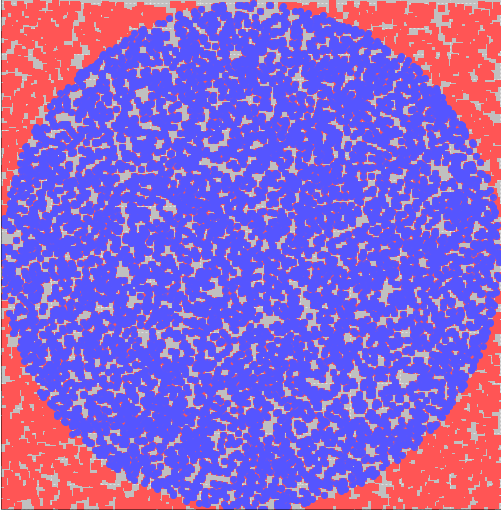
\includegraphics[scale=0.25]{monteCarlo.png}
\label{monte}
\caption{Les points bleues représentent les issues dans le disque et les points rouges à l'extérieur}
\end{figure}
La méthode pour estimer $\pi$ consiste alors à tirer au hasard des nombres $x$ et $y$ dans l'intervalle $[-1,1]$ ; 
si $x^2 + y^2 < 1$ le point $M(x,y)$ appartient au disque de rayon 1. On utilise la commande uniform(-1,1) pour générer une variable aléatoire suivant la loi uniforme dans le segment $[-1,1]$. On répète cette expérience un grand nombre de fois pour estimer $\mathbb{P}$("Flèche dans disque") et ainsi estimer $\pi$. 
\begin{enumerate}
\item \textbf{Tirer} : écrire une fonction lancerFleche(n) qui génère un couple de variables aléatoires suivant la loi uniforme dans le segment $[-1,1]$  
\item \textbf{Tester dans disque} : écrire une fonction dansDisque(x,y)
qui renvoie True ou False selon que la flèche de coordonnées (x,y) est dans le disque.
\item  \textbf{Estimer $\mathbb{P}$("Flèche dans disque")} : en utilisant les deux questions précédentes, écrire une fonction probaDisque(nbrexp)
qui estime $\mathbb{P}$("Flèche dans disque") par le principe de Monte-Carlo en réalisant l'expérience nbrexp fois
\item \textbf{Estimer $\pi$} : donner une approximation de $\pi$.
\end{enumerate}

\end{document}
